\chapter{МОДЕЛИРОВАНИЕ ГОРЯЧЕЙ ПЛАЗМЫ В ОТКРЫТОЙ МАГНИТНОЙ ЛОВУШКЕ}


Посчитанные примеры в главе \ref{ch4} служат доказательством того, что расчётная программа написана правильно и может использоваться для более сложных расчётов.

Применим построенную модель для расчёта реальной системы, для которой имеется ряд экспериментальных данных. В качестве такой системы выберем установку ГДЛ --- это установка для удержания субтермоядерной плазмы открытого типа. В работе \cite{anikeev2012} представлены результаты экспериментов 2012 года, когда на установку установили компактные пробкотроны вместо обычных магнитных пробок. Далее весь сравнительный анализ будет производится именно с данным источником.

\section{Общие сведения об установке ГДЛ}

Установка ГДЛ (рисунок \ref{fig:GDL2012}) представляет собой большой камеру длиной порядка $L = 7 \text{ м}$ и радиусом около $R = 0.7 \text{ м}$. Камера имеет сужения в двух торцевых частях, где как раз располагаются компактные пробкотроны. В средней части эквидистантно находятся 12 магнитных катушек. Магнитная система представлена на рисунке \ref{fig:beutyB}.  

Кроме всего этого установка богата различными датчиками и системами регистрирования. Возможно замерять плотности плазмы, ионную и электронную температуру и многое другое. Однако, подробное описание всех регистрирующих систем выходит за рамки данной работы.

Уставка имеет несколько источников нагрева плазмы:
\begin{enumerate}
	\item Инжекция горячих нейтралов в центральную часть с помощью 6-ти инжекторов. Мощность каждого инжектора составляет $P = 0,5 \text{ МВт}$. Расположены они под углом $45^{\circ}$ к главной оси симметрии. Важно заметить, что отсутствует полная симметрия вращения --- в силу технических особенностей инжекторы отсутствуют сверху и снизу установки.
	\item СВЧ нагрев на циклотронной частоте. Не учитывается в данной работе.
\end{enumerate}

\begin{figure}[h!]
	\centering
	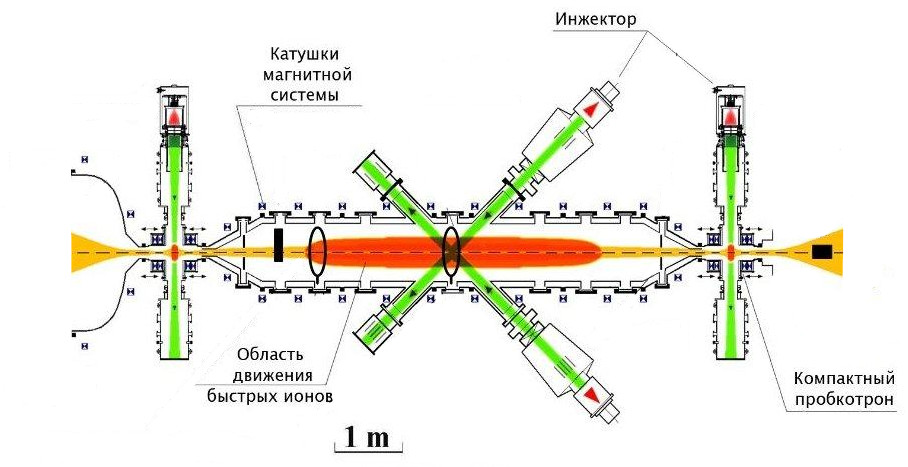
\includegraphics[width=0.9\linewidth]{../fig/ch5/GDL2012}
	\caption{Упрощённая схема экспериментальной установки ГДЛ, с установленными на ней компактными пробкотронами.}
	\label{fig:GDL2012}
\end{figure}
\begin{figure}[h!]
	\centering
	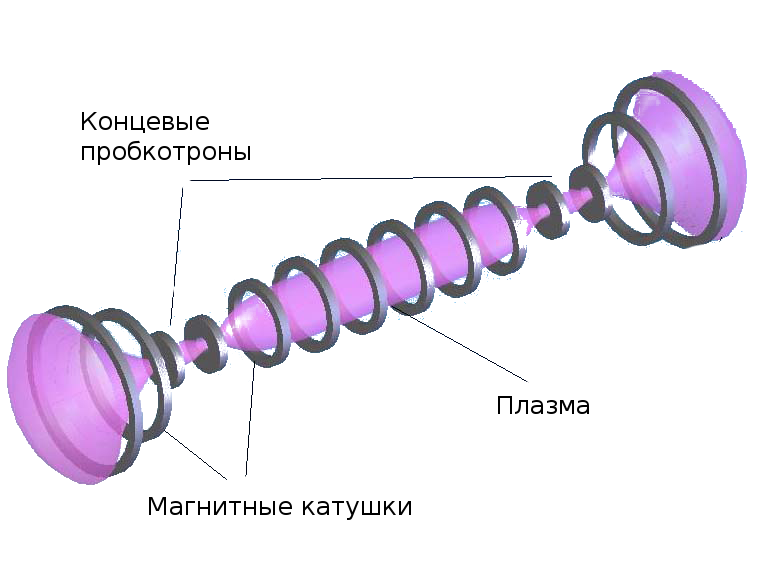
\includegraphics[width=0.6\linewidth]{../fig/ch5/beutyB}
	\caption{Упрощённая схема магнитной системы установки ГДЛ}
	\label{fig:beutyB}
\end{figure}

Одной из основных проблем удержания плазмы в открытых ловушках является продольные потери. Механизм этого явления следующий. Дрейфовая теория движения заряженных частиц в магнитном поле открытой ловушке гласит \cite{kotelnikov}, что факт удержания частицы происходит, если выполняется условие
\begin{equation}
	\frac{v_{\perp}^2(\vec{r})}{v^2(\vec{r})} > \frac{B(\vec{r})}{B_{\max}},
\end{equation}
где $v_{\perp}$ --- перпендикулярная линии магнитного поля составляющая скорости. 
Стоить отметить, что угол $\vartheta$, который даётся как
\begin{equation}
	\sin \vartheta = \frac{v_{\perp}}{v} = \sqrt{\frac{B_{\min}}{B_{\max}}}
\end{equation}
определяет так называемый конус потерь. 
Таким образом, частица, испытав рассеяние, может изменить $v_{\perp}$ и попасть тем самым в конус потерь. Средняя скорость движения электронов и ионов различается в $\bar{v}_e/\bar{v}_i \sim 10^3$. Вероятность за один и тот же промежуток времени того, что электрон попадёт в конус потерь получается большей, поэтому продольные электронные потери гораздо выше, чем ионные. Данный факт подтверждается экспериментально. А если это так, то на концах установки образуется нескомпенсированный положительный заряд, который <<выталкивает>> рядом находящееся ионы, тем самым ещё сильнее увеличивая потери.

Для борьбы с данным эффектом в ГДЛ было предложено \cite{anikeev2012} установить компактные пробкотроны вместо обычных магнитных зеркал. В данные пробкотроны с небольшим пробочным отношением ($R \approx 2$) инжектируются положительные заряженные ионы, которые создают положительный амбиполярный потенциал на концах установки, который значительно препятствует выходу ионов из центральной части.

\section{Постановка численного эксперимента}

\subsection{Упрощения и допущения модели}

Приблизим численную модель как можно ближе к реальной установке. Причём постараемся выделить наиболее значительные физические явления и процессы для описания системы в течении продолжительного промежутка времени --- $T = 10 \text{ мс}$.

В силу особенностей выбранного численного метода (метод <<частица-частица>>), вытекают некоторые ограничения и упрощения:
\begin{enumerate}
	\item Решение несамосогласованной задачи. Внешнее магнитное поле рассчитывается один раз и считается стационарным в течение всего времени моделирования. Движение плазмы никак на внешнее поле не влияет. Это упрощение вполне допустимо, учитывая безинерционный режим работы установки.
	\item Расчёт только ионов. Наличие электронного газа учитывается с помощью дебаевской экранировки \eqref{eq:debai1}. Таким образом, силы пространственного взаимодействия будут вычисляться согласно выражению \eqref{eq:force_with_debai}. Данное упрощение приходится делать по двум основным причинам: во-первый, время дискретизации при учёте электронов уменьшится на 4 порядка; во-вторых, количество частиц для адекватного описания системы становится огромным. Как следствие, вычисления становятся слишком трудоёмкими.
	\item Учитывая соотношение $\dfrac{r_D}{L} \ll 1$, можно вообще отказаться от сил пространственного взаимодействия. Действительно, использовав данные из раздела \ref{sec:open_trap}, согласно формуле \eqref{eq:debai_analitic},  получим
	\begin{equation*}
		r_D \sim 10^{-4} \text{ м} \qquad \to \qquad \frac{r_D}{L} \sim 10^{-5}.
	\end{equation*}
	\item Пренебрежение процессами ионизации и термоядерного синтеза.
	\item Влияние стенок на движение ионов отсутствует.
\end{enumerate}

Далее, остановимся на некоторых конкретных задачах, которые возникли в процессе создания численной модели.

\subsection{Расчёт магнитного поля}

Считая магнитные катушки достаточно тонкими, в данной модели они были замены кольцами с током. Создав такую систему колец, радиусы которых равны радиусами реальных магнитных катушек в установке. 

Зададим расположения контуров с током (таблица 4.1).
Далее, основная сложность заключается в подборе эквивалентных токов $I_i$ каждого из колец.

\begin{table}[h!]
	\center
	\parbox{10.7cm}{
		\caption{Параметры контуров с током}
	}
	\begin{tabular}{c|c|c|c}\label{tab:currents}
		№  & Координата $z_i$, м & Радиус $R_i'$, м & Ток $I_i$, А  \\ \hline \hline
		1  & -3,50  & 0,3  & 0.50$\cdot10^7$ \\
		2  & -3,96  & 0,3  & 0.49$\cdot10^7$ \\
		3  & -3     & 0,45 & 2$\cdot10^6$ \\
		4  & -2,5   & 0,7  & 2$\cdot10^6$ \\ 
		5  & -1,944 & 0,7  & 1$\cdot10^6$ \\ 
		6  & -1,389 & 0,7  & 1$\cdot10^6$ \\
		7  & -0,833 & 0,7  & 7$\cdot10^5$ \\
		8  & -0,278 & 0,7  & 7$\cdot10^5$ \\ 
		9  & 0,278  & 0,7  & 7$\cdot10^5$ \\ 
		10 & 0,833  & 0,7  & 7$\cdot10^5$ \\ 
		11 & 1,389  & 0,7  & 1$\cdot10^6$ \\ 
		12 & 1,944  & 0,7  & 1$\cdot10^6$ \\
		13 & 2,5    & 0,7  & 2$\cdot10^6$ \\
		14 & 3,0    & 0,45 & 2$\cdot10^6$ \\
		15 & 3,50   & 0,3  & 0.5$\cdot10^7$ \\
		16 & 3,96   & 0,3  & 0.49$\cdot10^7$ \\
	\end{tabular}
	\label{tab:prm}
\end{table} 

Численный расчёт модуля магнитной индукции производится следующим образом. Пусть есть только одно кольцо радиусом $R_k'$ и $z$-координатой $z_k$ с током $I_k$. Пространство разбивается на прямоугольную сетку. Выбирается один из узлов с координатами $\vec{r}_n = \left\{ x_n;y_n;z_n \right\}$. Переход в цилиндрическую систему координат позволяет свести промежуточную задачу к двухмерной 
\begin{equation}
	\rho_n = \sqrt{x_n^2 + y_n^2}, \qquad z_n = z_n.
\end{equation}
Далее требуется найти вектор магнитной индукции $\vec{B}_k = \left\{ B^{\rho}_k; B_k^z \right\}$, причём необходимо учесть, что её модуль определяется согласно формуле \eqref{eq:calcBcyl}, а направление согласно правилу правого винта:
\begin{eqnarray}
	B^{\rho}_k &=& \frac{\mu_0 R_k'}{2} \frac{I_k \left( R_k' - \rho_n \right)}{\left( \left( R_k' - \rho_n \right)^2 + \left( z_k - z_n \right)^2 \right)^{3/2}}, \\ \nonumber \\ \nonumber \\
	B^{z}_k &=& \frac{\mu_0 R_k'}{2} \frac{I_k \left( z_k - z_n \right)}{\left( \left( R_k' - \rho_n \right)^2 + \left( z_k - z_n \right)^2 \right)^{3/2}}.
\end{eqnarray}
В силу суперпозиции, магнитная индукция от всех контуров с током в системе будет вычисляться как $\vec{B}_n = \sum \vec{B}_k$. Перейдя в декартову систему координат, получим окончательные значения компонент вектора $\vec{B}(\vec{r}_n)$. Данный алгоритм необходимо повторить для каждого узла сетки.

\begin{figure}[h]
	\begin{minipage}[h]{0.9\linewidth}
		\center{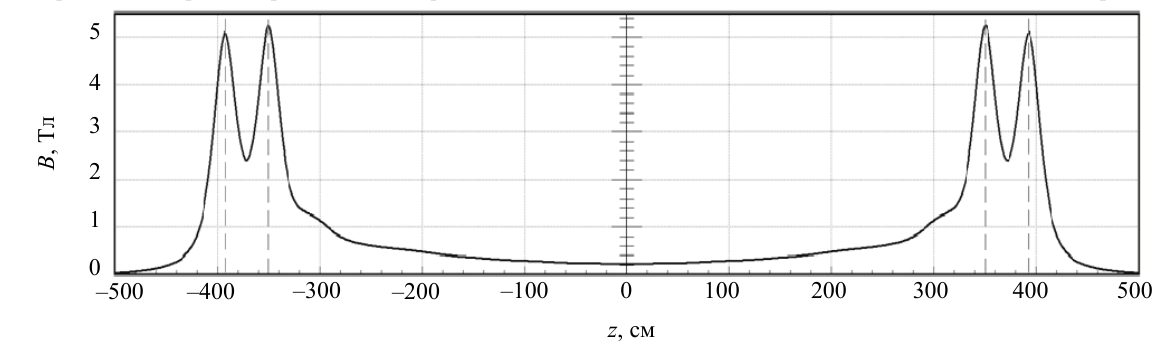
\includegraphics[width=0.9\linewidth]{fig/ch5/B_article} \\ а) Из экспериментальной работы \cite{anikeev2012}}
	\end{minipage}
	\vfill
	\begin{minipage}[h]{0.9\linewidth}
		\center{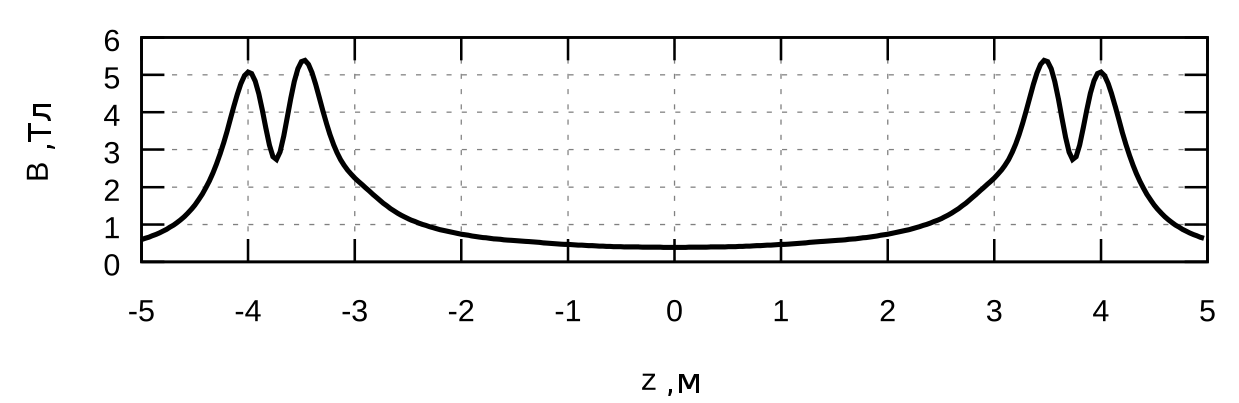
\includegraphics[width=0.91\linewidth]{fig/ch5/myB} \\ б) Из полученной модели}
	\end{minipage}
	\caption{Зависимость модуля индукции магнитного поля на оси симметрии установки}
	\label{fig:B_on_axis}
\end{figure}
\begin{figure}[h!]
	\centering
	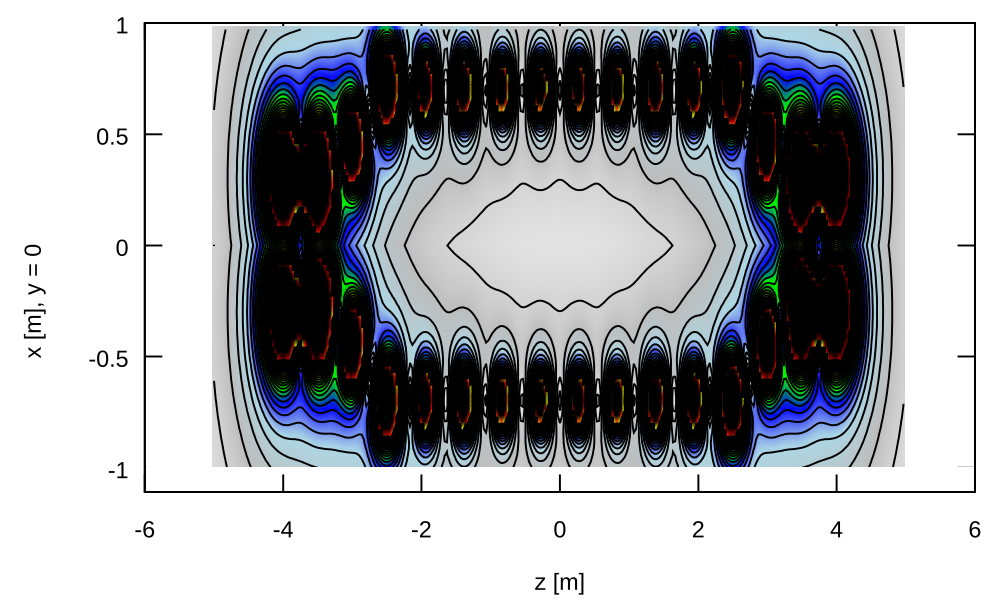
\includegraphics[width=0.8\linewidth]{fig/ch5/mymapB_fine}
	\caption{Карта магнитного поля установки, полученное из представленной модели}
	\label{fig:mymapB_fine}
\end{figure}

Существует экспериментально снятая зависимость $B(z)$ на оси симметрии установки (рисунок \ref{fig:B_on_axis}, а). Варьируя $I_i$, получим необходимый результат (рисунок \ref{fig:B_on_axis}, б). Численная реализация данного расчёта позволяет также получить и карту изолиний $\vec{B}$ (рисунок \ref{fig:mymapB_fine}).


\subsection{Расчёт ионов в полученной системе}

В данном исследовании считается, что мишенная плазма уже есть в установке и предварительный СВЧ нагрев был произведён. Плазма представляет собой однократно ионизированные атомы дейтерия:
\begin{equation}
	m_D = 3,344\cdot10^{-27} \text{ кг}, \qquad q_D = + 1,602 \cdot 10^{-19} \text{ Кл}.
\end{equation}

В силу малого количество информации о равновесном состоянии плазмы, было принято поступить следующим образом. Инициализация плазмы, а точнее ионов, происходит равномерно случайным образом в объёме цилиндра с параметрами
\begin{equation}
	R_{born} = 0,15 \text{ м}, \qquad L_{born} = 6 \text{ м}.
\end{equation} 
Тогда концентрацию в начальный момент времени можно записать, как
\begin{equation}
	n_i(x,y,z) = 
	\begin{cases}
		n_0, & \text{ если }\begin{cases}
		\sqrt{x^2 + y^2} < R_{born}, \\
		\frac{L_{born}}{2} < z < \frac{L_{born}}{2},
		\end{cases} \\
		0,   & \text{ иначе},
	\end{cases}
\end{equation}
где $n_0 = 10^{20} \text{ м}^{-3}$.
Данные параметры взяты из \cite{anikeev2012}, однако, при таком выборе отсутствует более подробная информация о функции концентрации $n_i(\vec{r})$. 

В качестве генератора случайных чисел выбран вихрь Мерсенна, о котором уже было сказано в разделе \ref{sec:MT19937}.

Начальные скорости мишенной плазмы задаются случайным образом с функцией распределения Максвелла \eqref{eq:maxwell_dist}. Подробно алгоритм численной реализации был описан в разделе \ref{sec:HowToMaxwell}.
Равновесная температура мишенной плазмы считалась равной $\bar{T}_{aim} = 1 \text{ кэВ}$.

В процессе моделирования могла происходить впрыск горячих нейтралов в центральную часть с помощью 6-ти инжекторов (рисунок \ref{fig:GDL2012}). Так как в модели не учитываются процессы ионизации нейтральных атомов при столкновениями с частицами плазмы, то вводится следующее предположение: ион дейтерия <<рождается>> вдоль оси инжекции случайным образом в области высокой концентрации мишенной плазмы.

Мощность каждого инжектора составляет 0,5 МВт при температуре частиц $T_{hot} = 20 \text{ кэВ}$. Схема расположения инжекторов показана на рисунке \ref{fig:gdl}. Инжекция начинается в момент времени $t_1 = 2  \text{ мс}$, а прекращается в момент $t_2 = 8 \text{ мс}$. Полное время моделирования составляет $T = 10 \text{ мс}$.

\begin{figure}[h!]
	\centering
	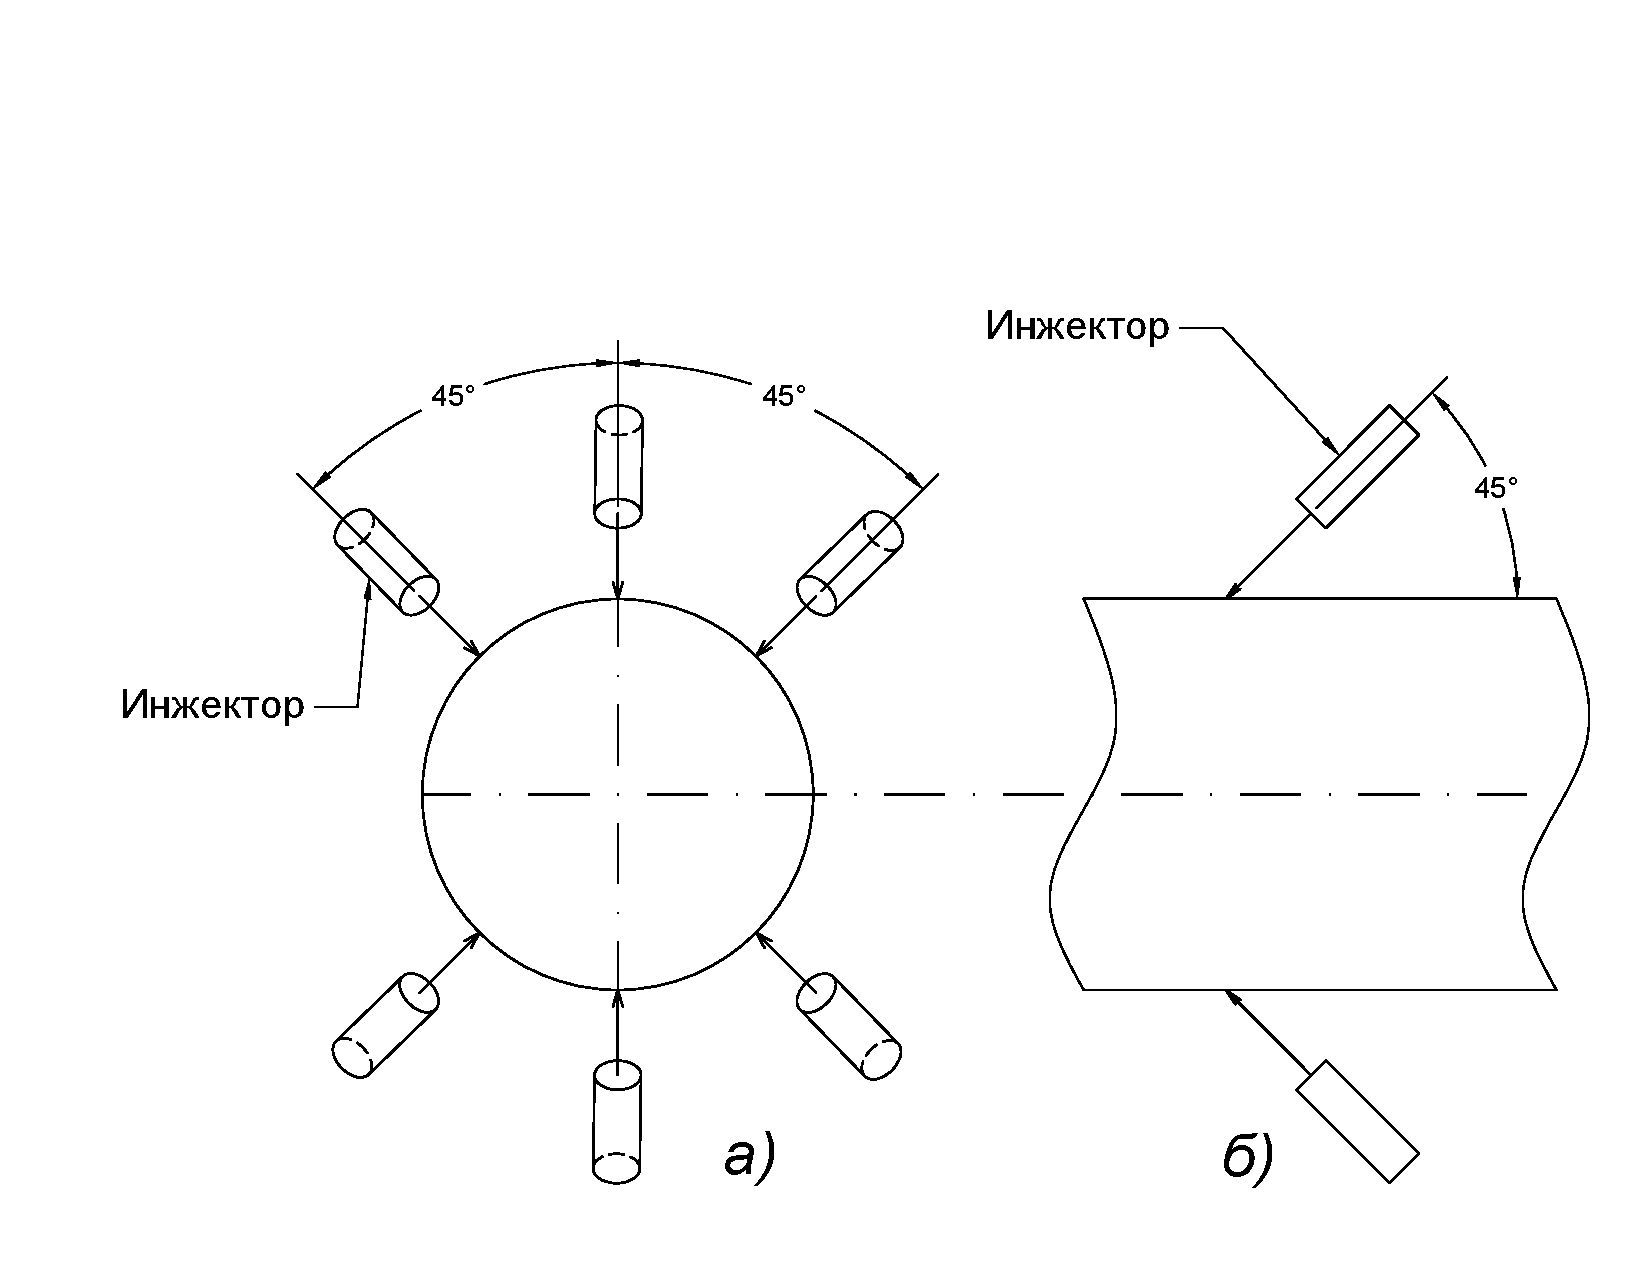
\includegraphics[width=1.\linewidth]{fig/ch5/gdl}
	\caption{Схематичное расположение инжекторов в установке ГДЛ: а) вид с торца; б) вид сбоку}
	\label{fig:gdl}
\end{figure}


\section{Результаты}

Было произведено несколько серий экспериментов. В каждой серии было от 7 до 10 численных расчёта с одинаковыми входными данными.
В каждом из экспериментов максимальное количество крупных частиц составляло $N = 55000$. Полученные данные были проанализированы и обработаны с помощью ряда программ, написанных на языке Python. Были вычислены средние значения
\begin{eqnarray}
	\bar{f} = \frac{1}{N_{exp}} \sum_{i = 1}^{N_{exp}} f_i 
\end{eqnarray}
и стандартные отклонения
\begin{eqnarray}
	\sigma_f = \sqrt{\frac{1}{N_{exp} - 1} \sum_{i = 1}^{N_{exp}} \left( f_i - \bar{f} \right)^2},
\end{eqnarray}
где $f$ --- интересующая величина, а суммирование ведётся по всем численным экспериментам с одинаковыми параметрами на входе.

\subsection{Эволюция распределений со временем}

Поскольку точные данные для корректной инициализации начальной мишенной плазмы получить практически невозможно, то необходимо проводить отдельные серии экспериментов для нахождения квазистационарных состояний системы. Для решения данной задачи очень важным является выяснить динамику изменений параметров.

Выбрав полное время моделирования $T = 10 \text{ мс}$, каждую 1 мс проанализируем состояние системы для определения $n(r)$ и $n(z)$. Усреднив полученные распределения, получим семейство линий, которые представлены на рисунке \ref{fig:density_evolution}.


\begin{figure}[H]
	\begin{minipage}[h]{0.99\linewidth}
		%\center{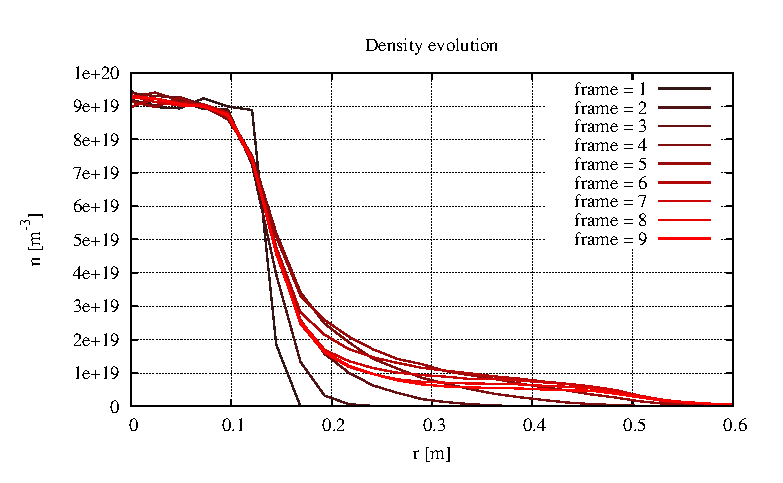
\includegraphics[width=0.9\linewidth]{fig/ch5/dt11-with_sources/eps/evolution/density_r_evo} \\ а) Эволюция радиальной плотности}
		\center{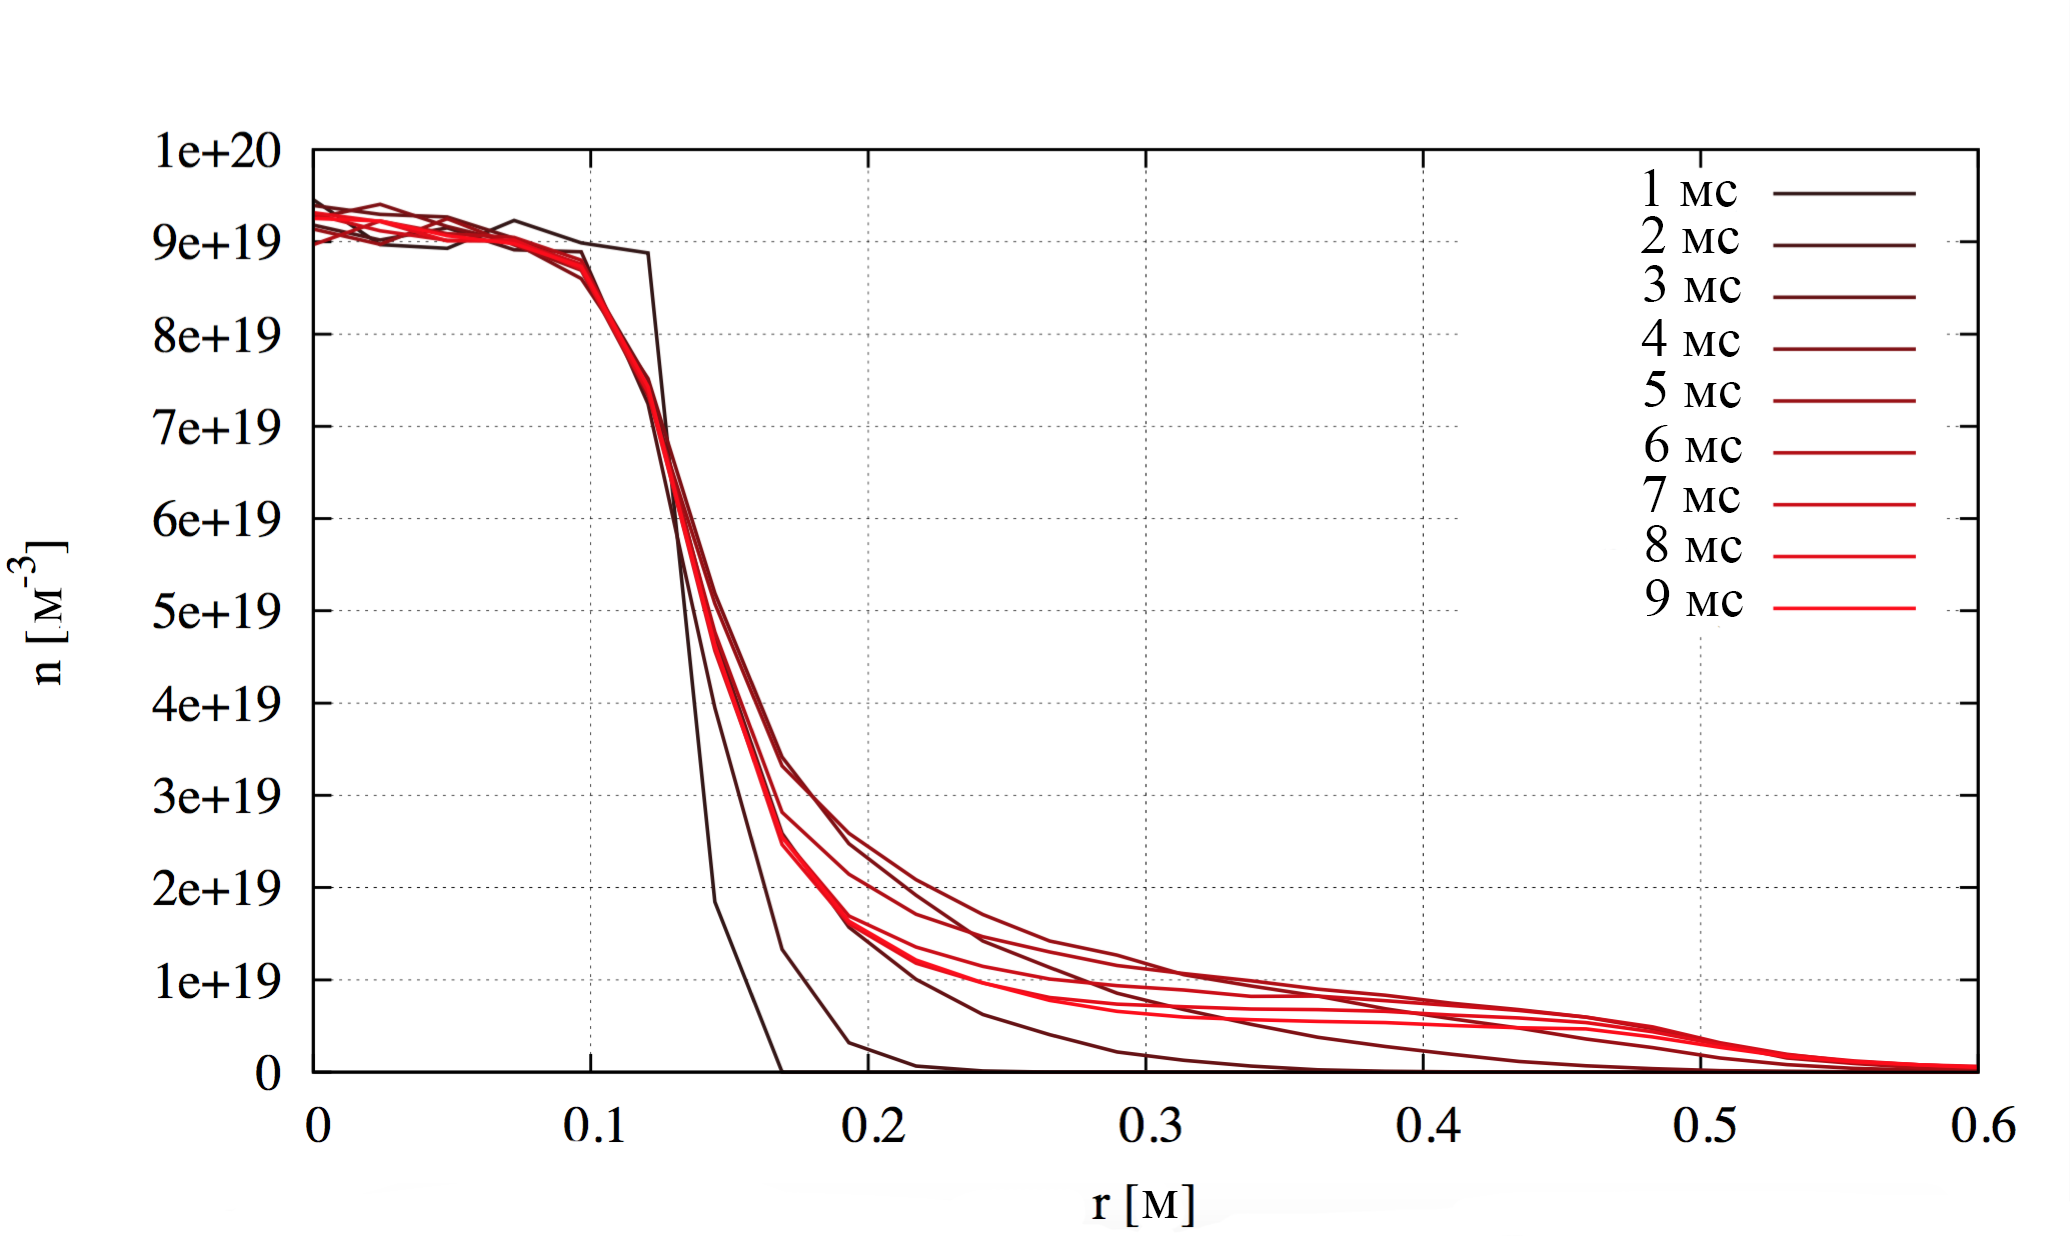
\includegraphics[width=0.9\linewidth]{fig/ch5/density_r_evo} \\ а) Эволюция радиальной плотности}
	\end{minipage}
	\hfill
	\begin{minipage}[h]{0.99\linewidth}
		%\center{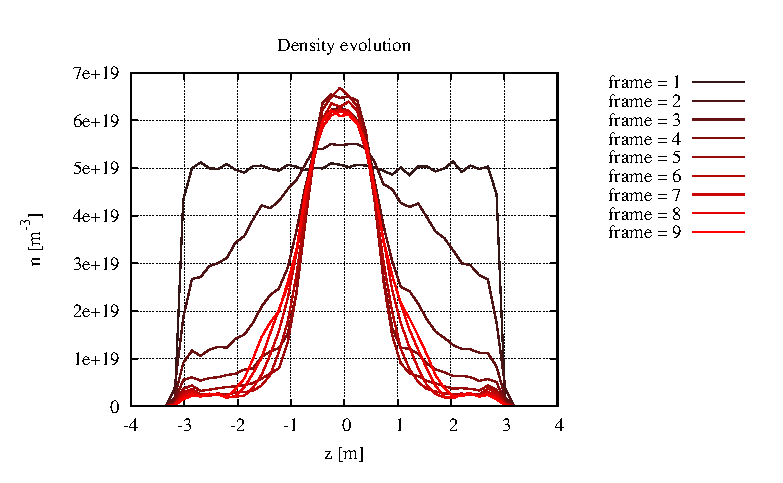
\includegraphics[width=0.9\linewidth]{fig/ch5/dt11-with_sources/eps/evolution/density_z_evo} \\ б) Эволюция линейной плотности}
		\center{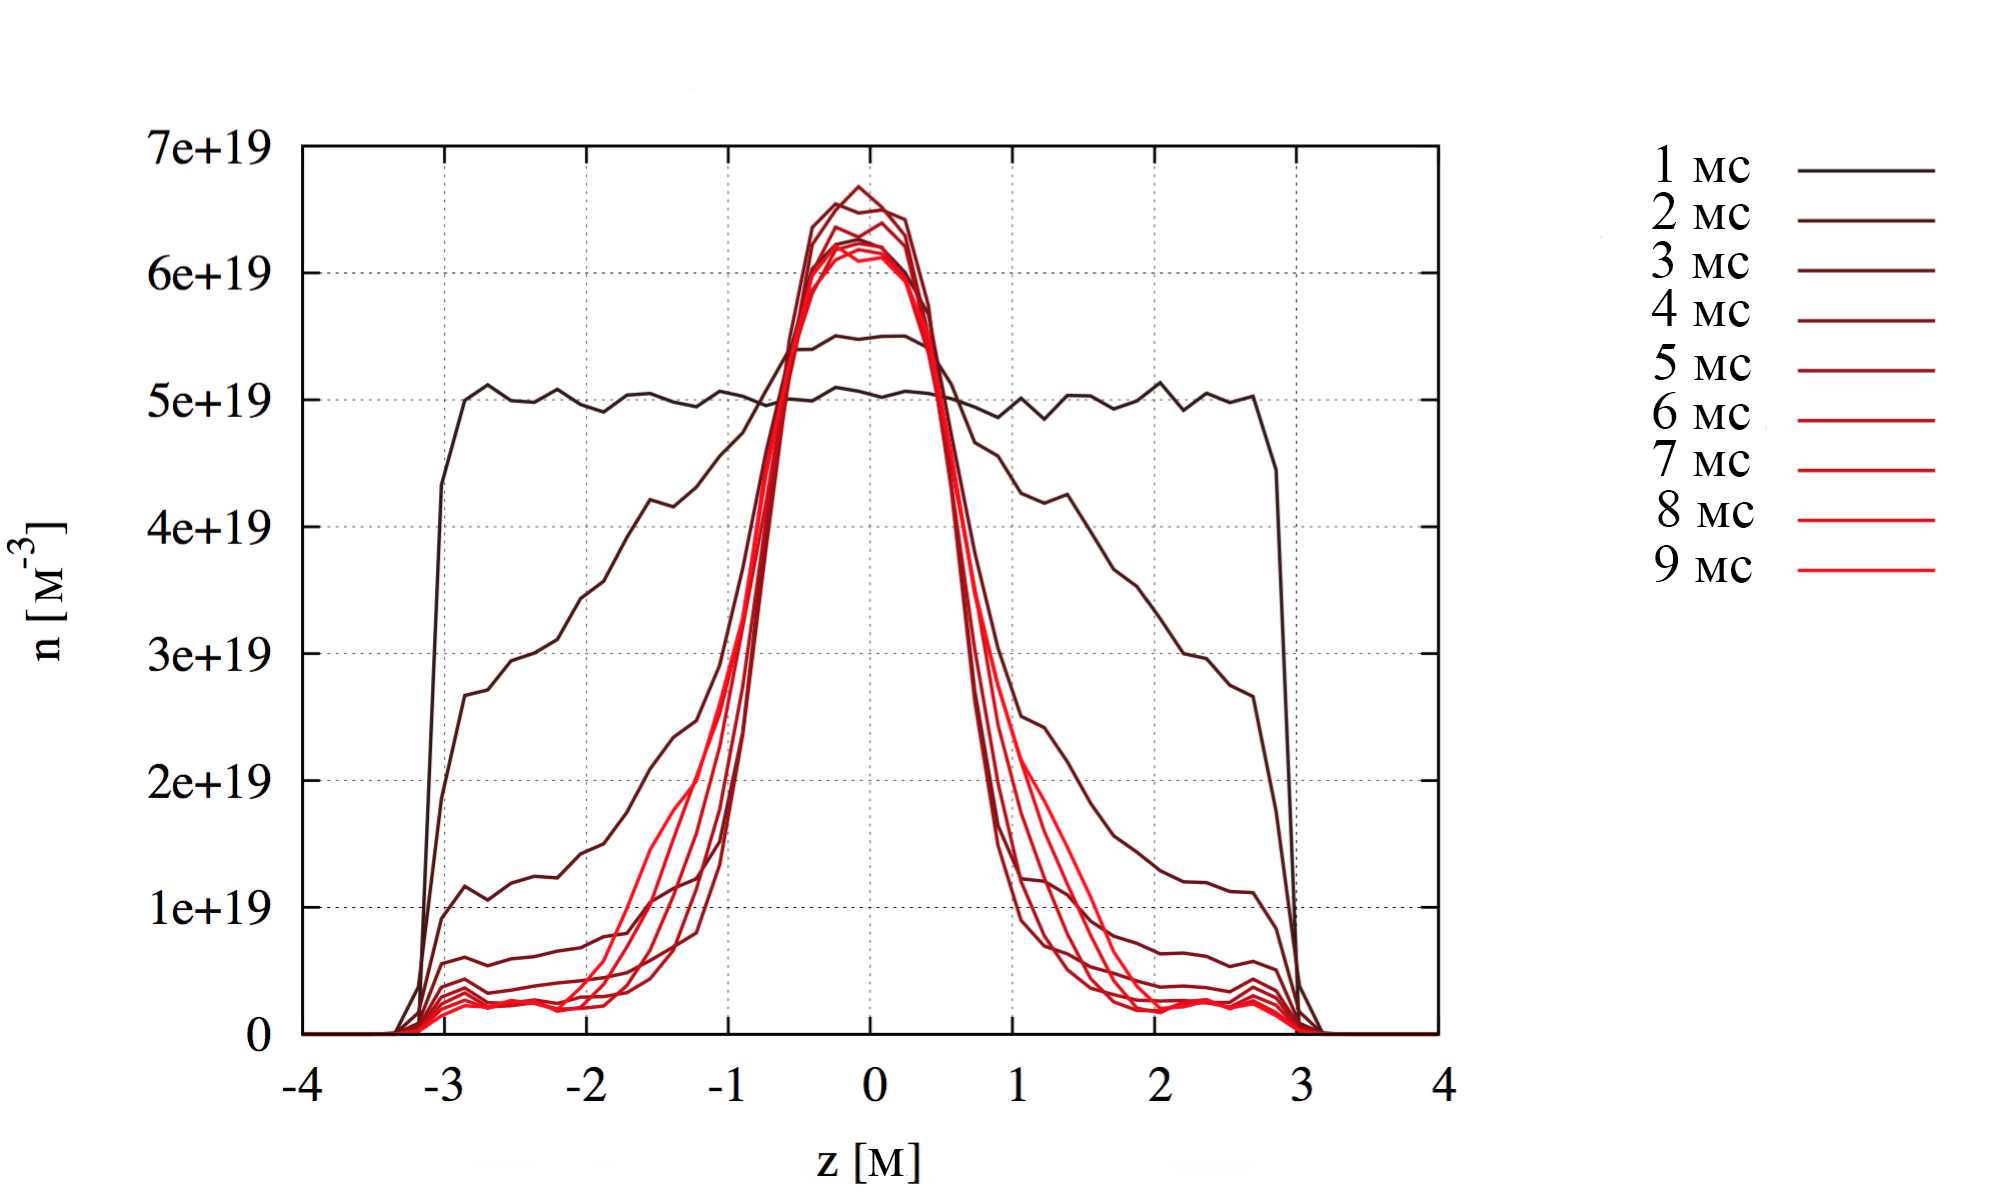
\includegraphics[width=0.9\linewidth]{fig/ch5/density_z_evo} \\ б) Эволюция линейной плотности}
	\end{minipage}
	\caption{Семейство линий, отображающих эволюцию плотности в установки с течением времени. Чем линия чернее, тем этот момент был раньше; чем линия краснее, тем ближе этот момент к окончанию моделирования}
	\label{fig:density_evolution}
\end{figure}

\subsection{Радиальная плотность}

У радиальной плотности наблюдается достаточно большое стандартное отклонение в центральной части (при $r = 0$), что видно на рисунке \ref{fig:density_r} а. Вполне может образовываться провал в этой области, причём как у горячих ($T_{hot} > 5 \text{ кэВ}$), так и у холодных ионов ($T_{aim} < 5 \text{ кэВ}$).

Учитывая большое среднеквадратичное отклонение в центральной части, можно сделать вывод о том, что там может образовываться неоднородность. Экспериментальные данные показывают качественно похожие результаты, что видно на рисунке \ref{fig:density_r} б.

Важно заметить, что с помощью составленной модели возможно определить ширину плазменного столба мз условия 
\begin{equation}
	n(r_p) = \frac{n_{\max}}{2} \qquad \to \qquad r_p \approx 0,15 \text{ м}.
\end{equation}
Эксперимент даёт значение $r_p^{exp} \approx 0,16 \div 0,18 \text{ м}$.

\begin{figure}[h!]
	\begin{minipage}[h]{0.49\linewidth}
		\center{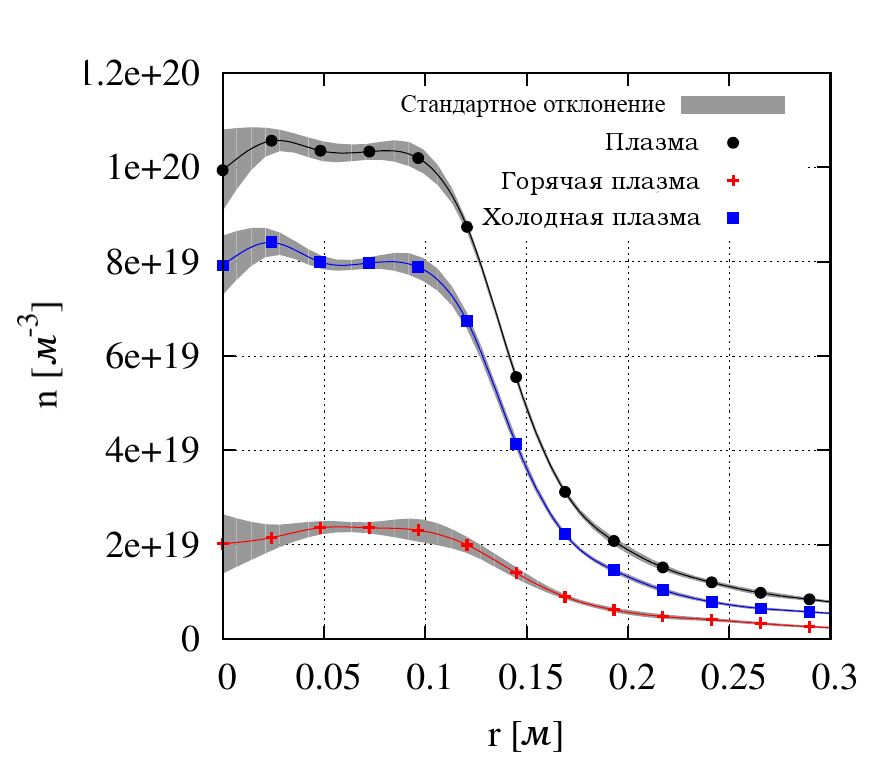
\includegraphics[width=1.08\linewidth]{fig/ch5/density_r} \\ а) Численный расчёт}
	\end{minipage}
	\hfill
	\begin{minipage}[h]{0.49\linewidth}
		\center{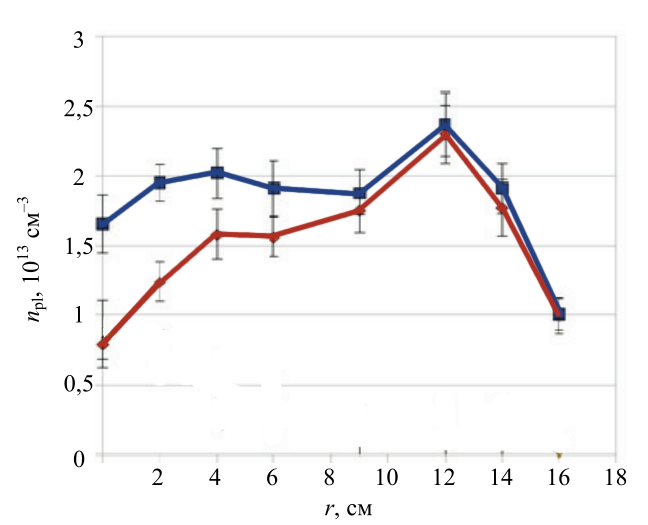
\includegraphics[width=1.1\linewidth]{fig/ch5/density_article} \\ б) Из работы \cite{anikeev2012}}
	\end{minipage}
	\caption{Радиальный профиль плотность плазмы при наличии инжекции. На рисунке б) $\blacksquare$ --- при дополнительной инжекции ионов в КП; $\blacklozenge$~---~без инжекции ионов в КП}
	\label{fig:density_r}
\end{figure}

\subsection{Линейная плотность}

График линейной плотности представлены на рисунке \ref{fig:density_z}. На нём видно, что из-за боковой инжекции пик плотности находится не по центру установки, а чуть смещён влево.

\begin{figure}[h!]
	\center
	%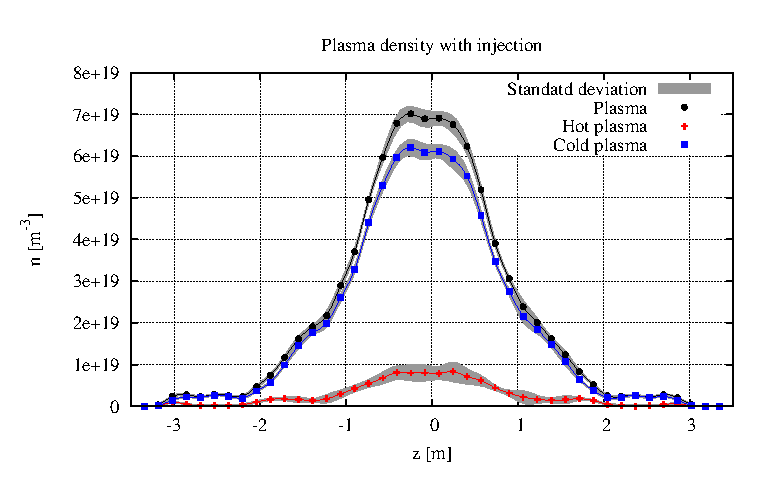
\includegraphics[width=1.\linewidth]{fig/ch5/dt11-with_sources/eps/density_z}
	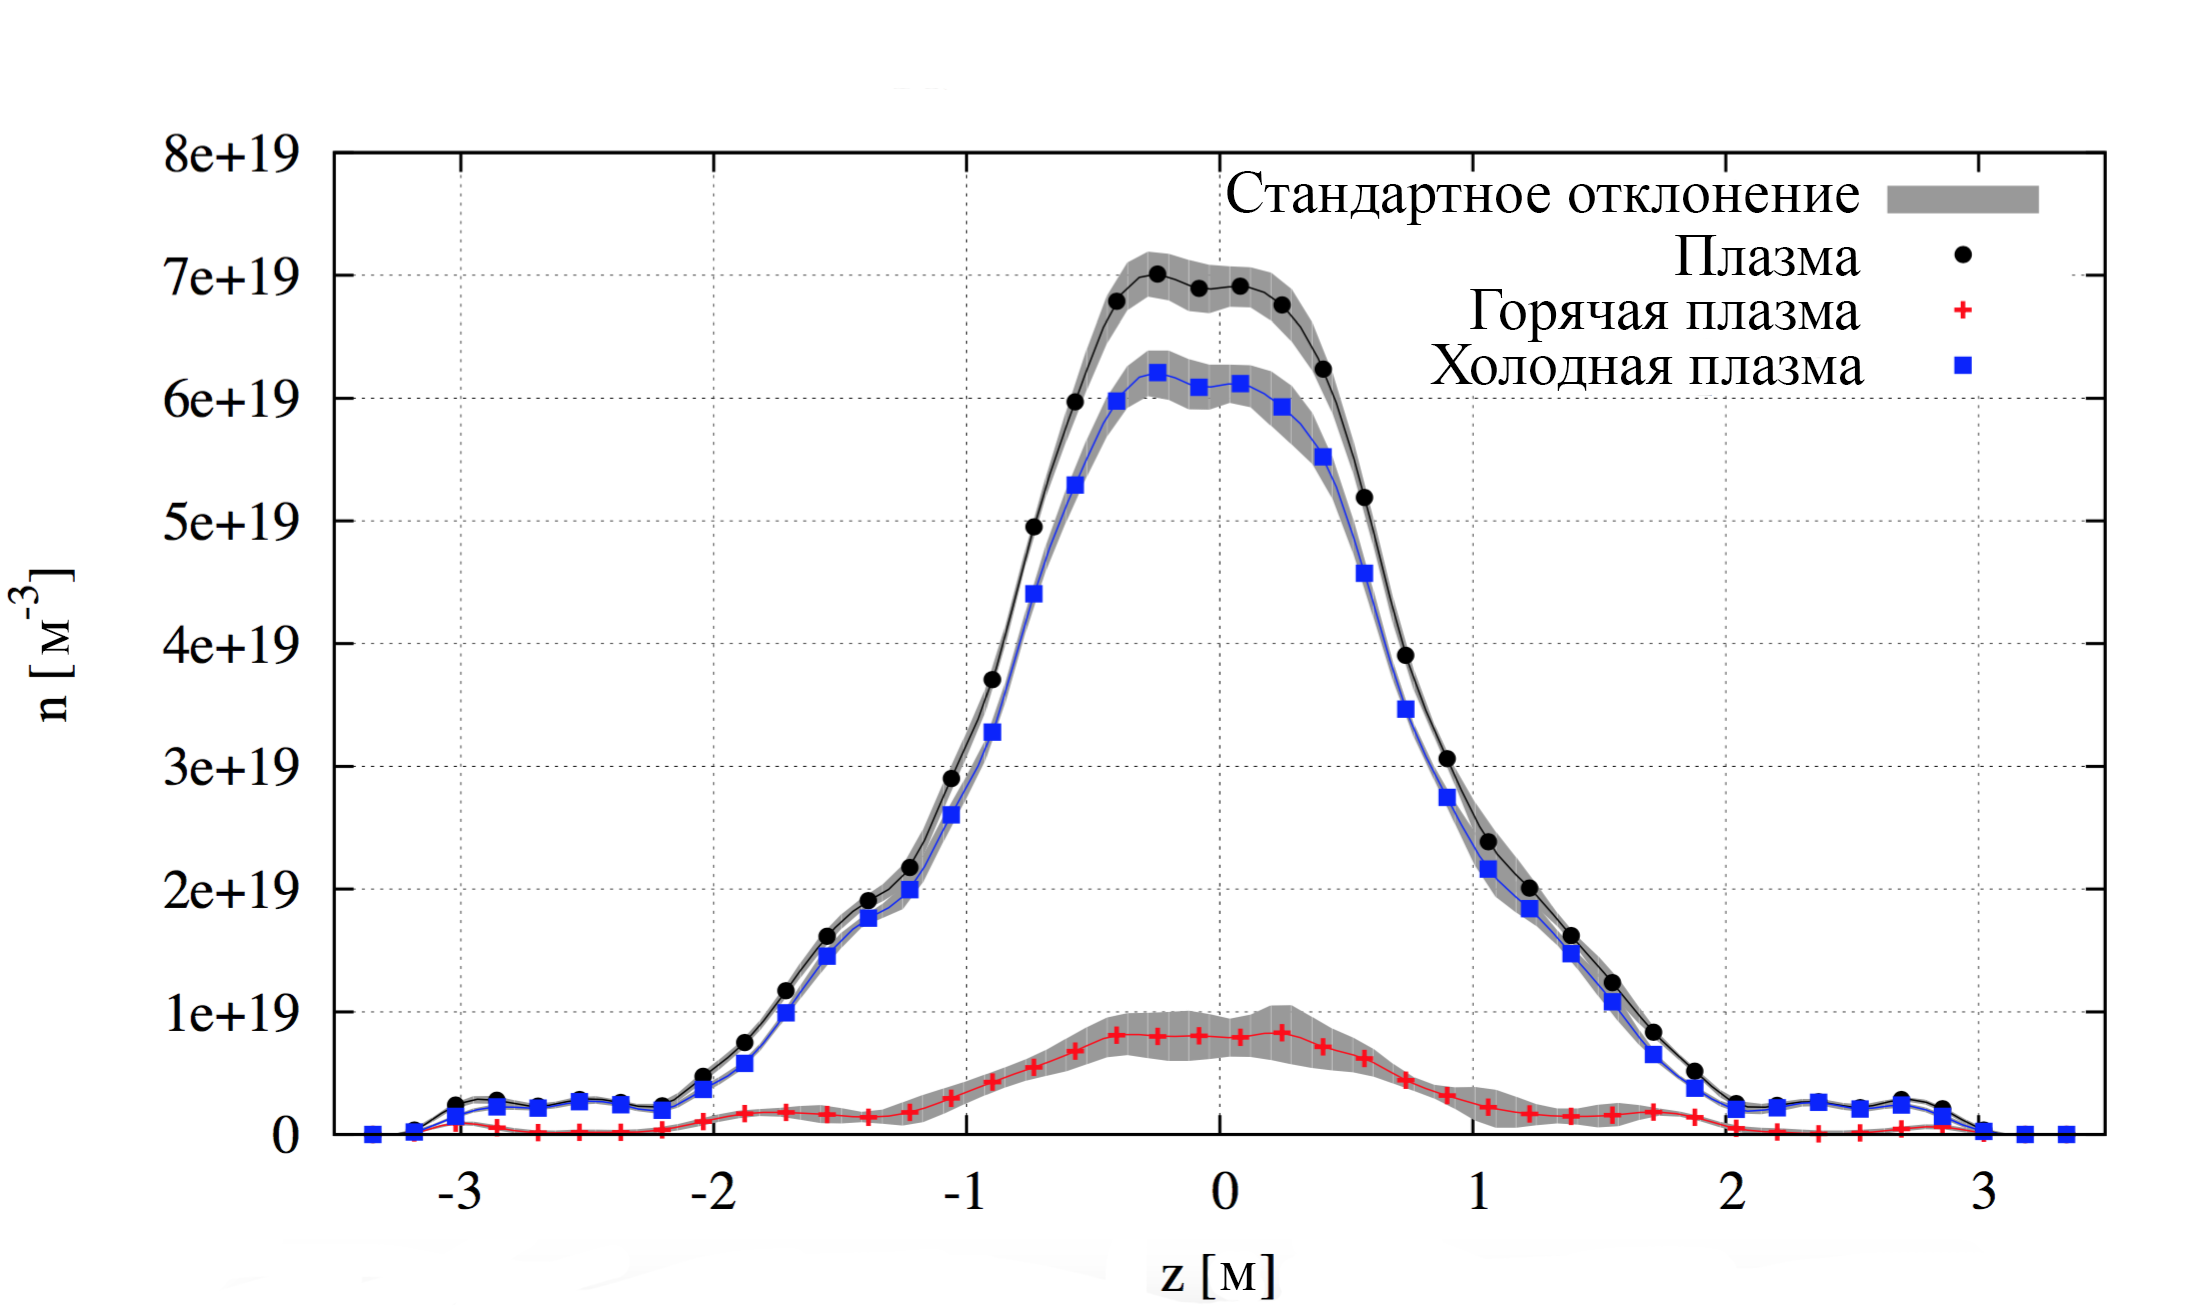
\includegraphics[width=1.\linewidth]{fig/ch5/density_z.png}
	\caption{Линейный профиль плотность плазмы при наличии инжекции}
	\label{fig:density_z}
\end{figure}

\subsection{Распределение температуры}

На графиках температуры уже явно видно, что при в областях с большей магнитной индукцией начинается расходимость. Также, анализируя графики а и б на рисунке \ref{fig:temperature}, необходимо принимать во внимание графики плотностей на рис. \ref{fig:density_r} и рис. \ref{fig:density_z} соответственно.

Проанализировав графики, можно сделать вывод о том, что температура слабо зависит от расстояния до оси симметрии. Однако, данный вывод расходится с экспериментальными наблюдениями --- температура, хоть и слабо, но убывает с увеличением расстояния до оси симметрии.

\begin{figure}[h!]
	\begin{minipage}[h]{0.89\linewidth}
		\center{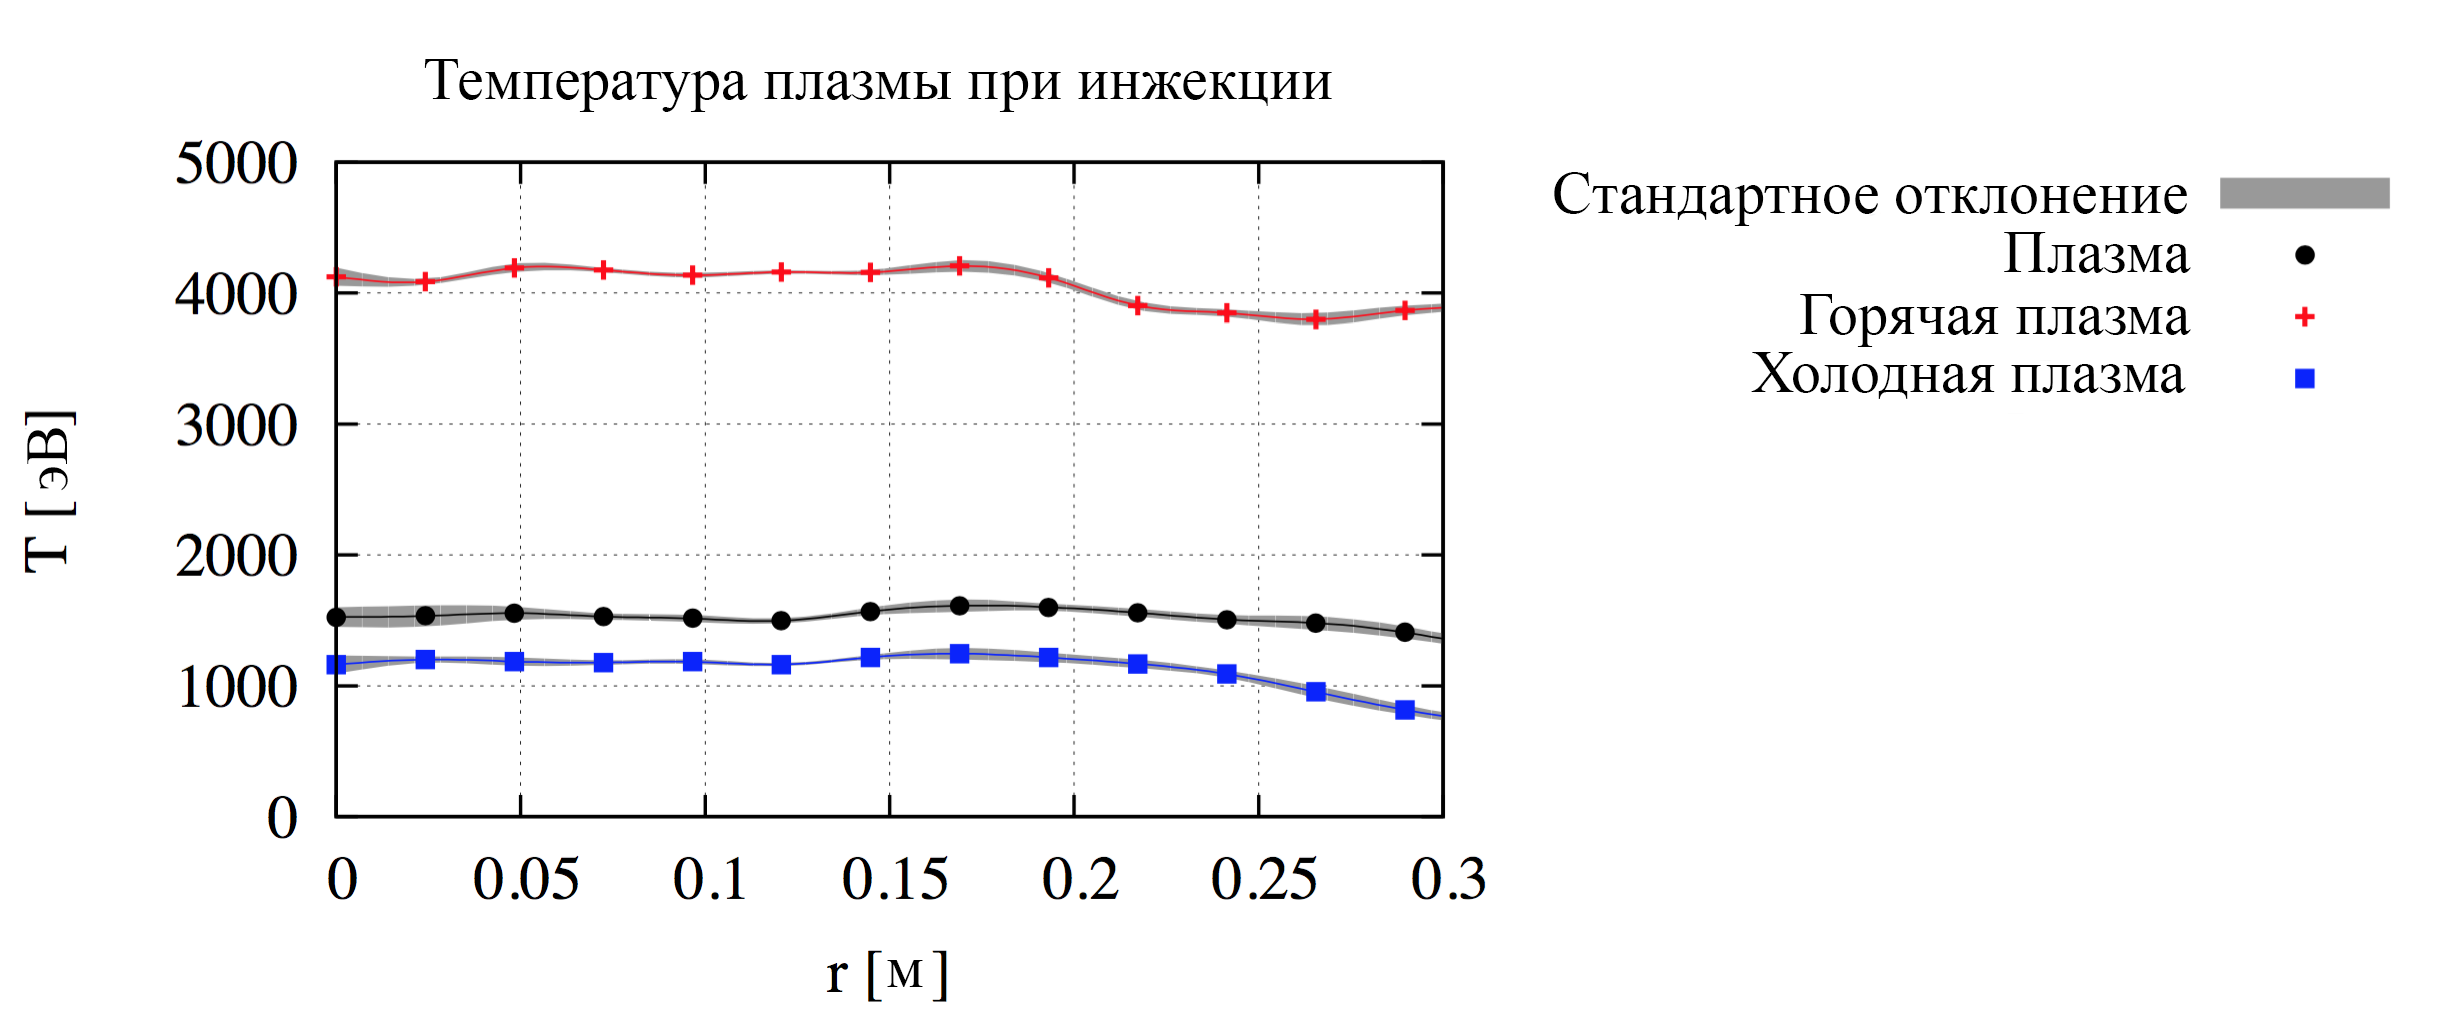
\includegraphics[width=1.1\linewidth]{fig/ch5/temperature_r.png} \\ \qquad \qquad а) }
	\end{minipage}
	\hfill
	\begin{minipage}[h]{0.89\linewidth}
		\center{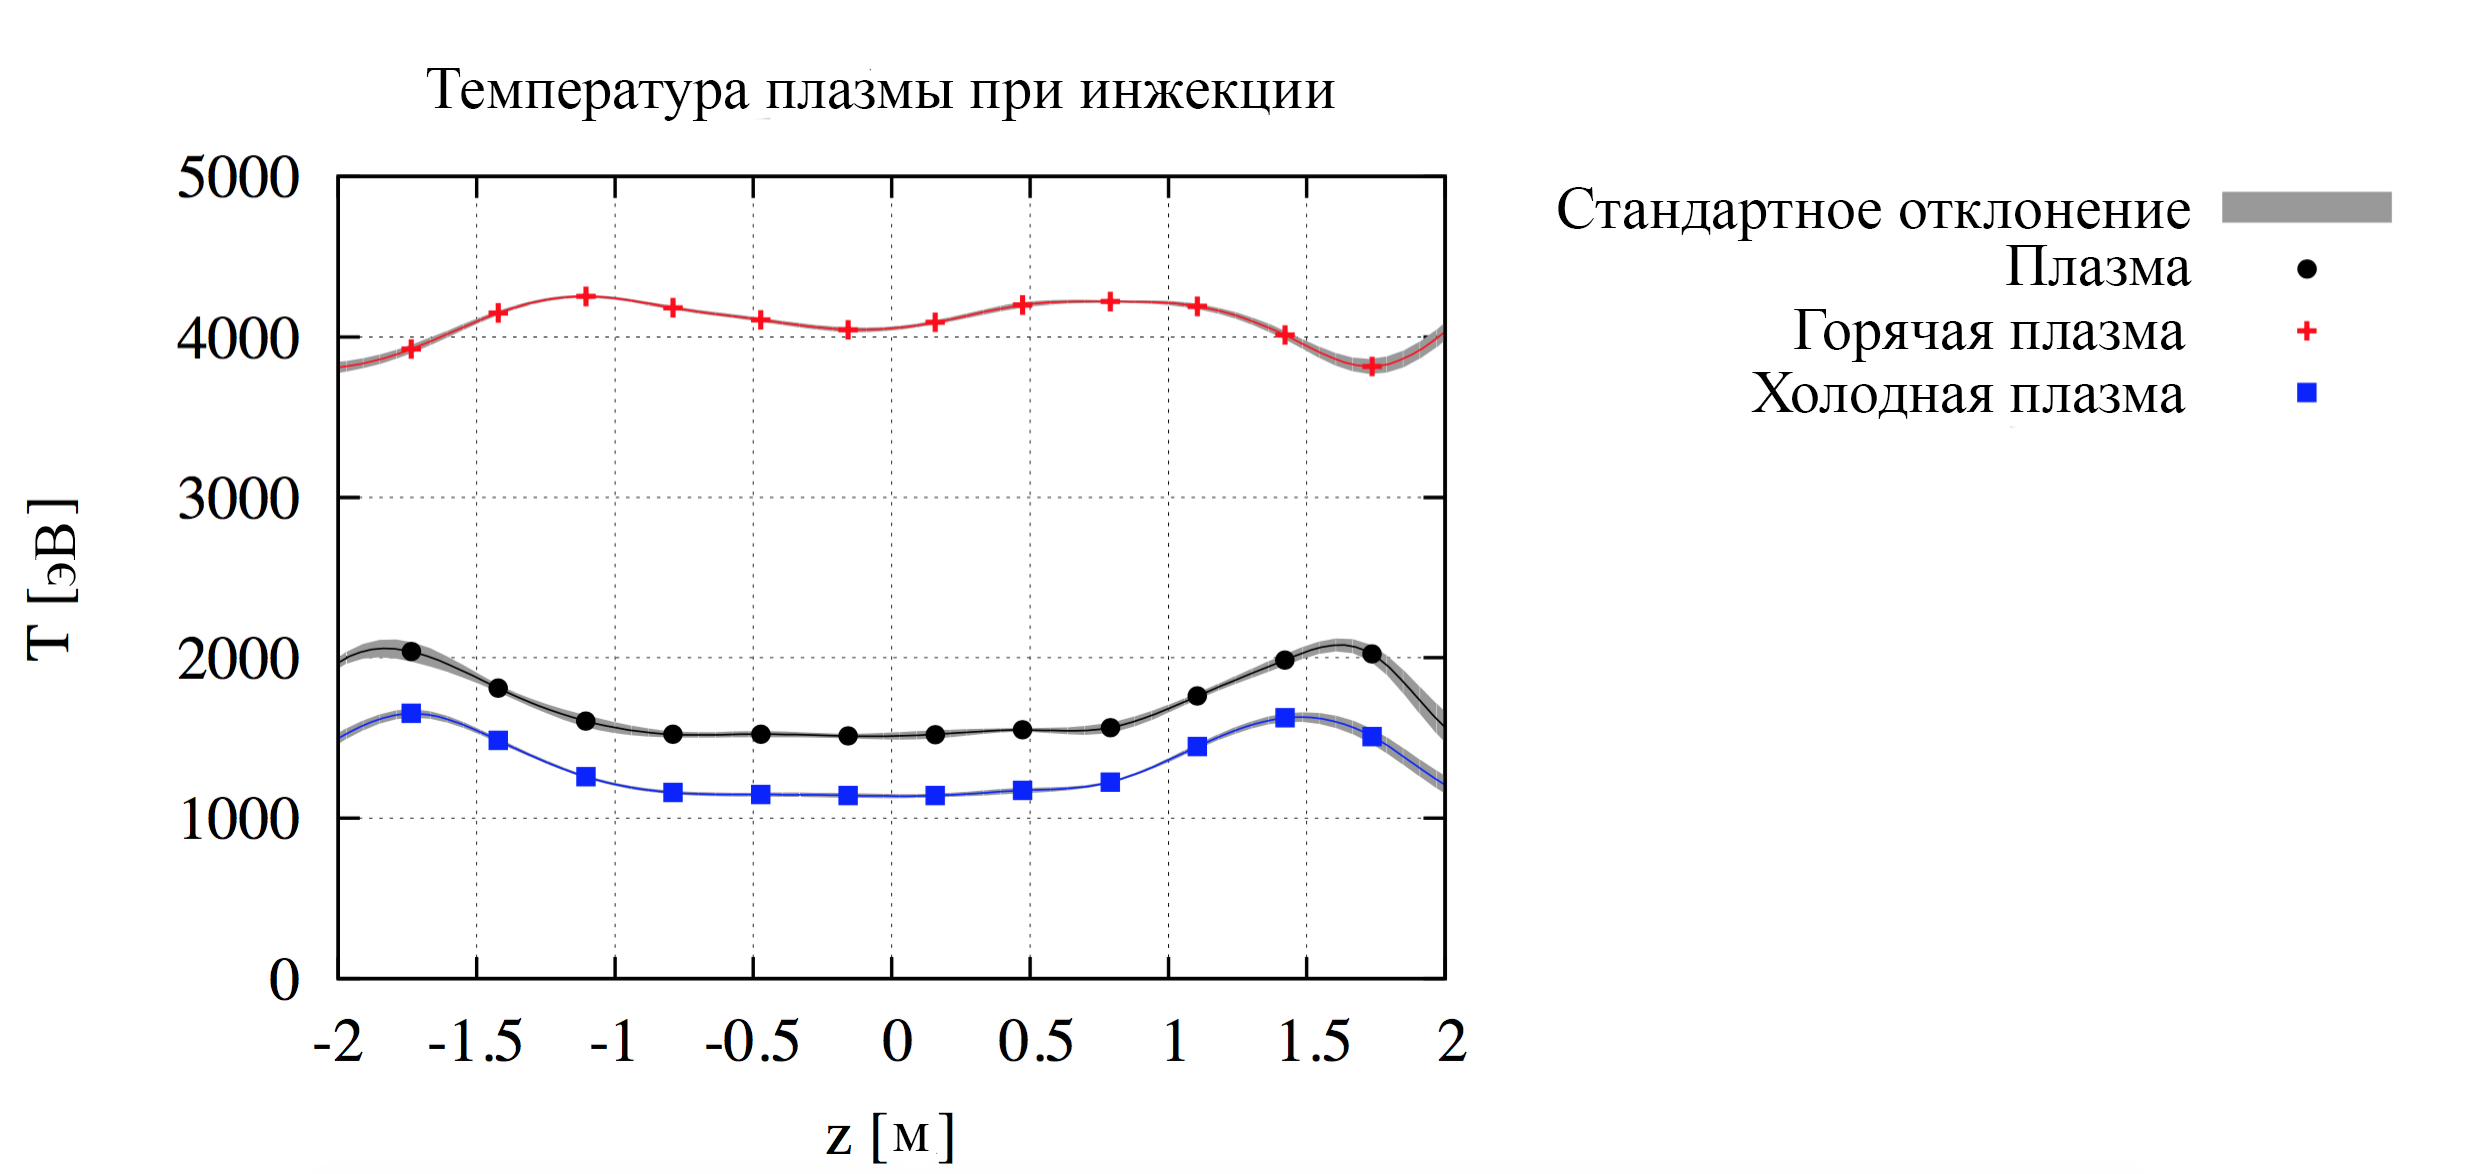
\includegraphics[width=1.1\linewidth]{fig/ch5/temperature_z.png} \\ \qquad \qquad б)}
	\end{minipage}
	\caption{Распределение температуры плазмы в установке: а) радиальное распределение; б) линейное распределение}
	\label{fig:temperature}
\end{figure}

\subsection{Распределение по скоростям}

Распределение по скоростям всегда получалось Максвелловским с хорошей степенью точности (типичная график представлен на рисунке \ref{fig:maxwell}). Причём никаких значительных отклонений в зависимости от места измерения тоже не было обнаружено.

\begin{figure}[h!]
	\centering
	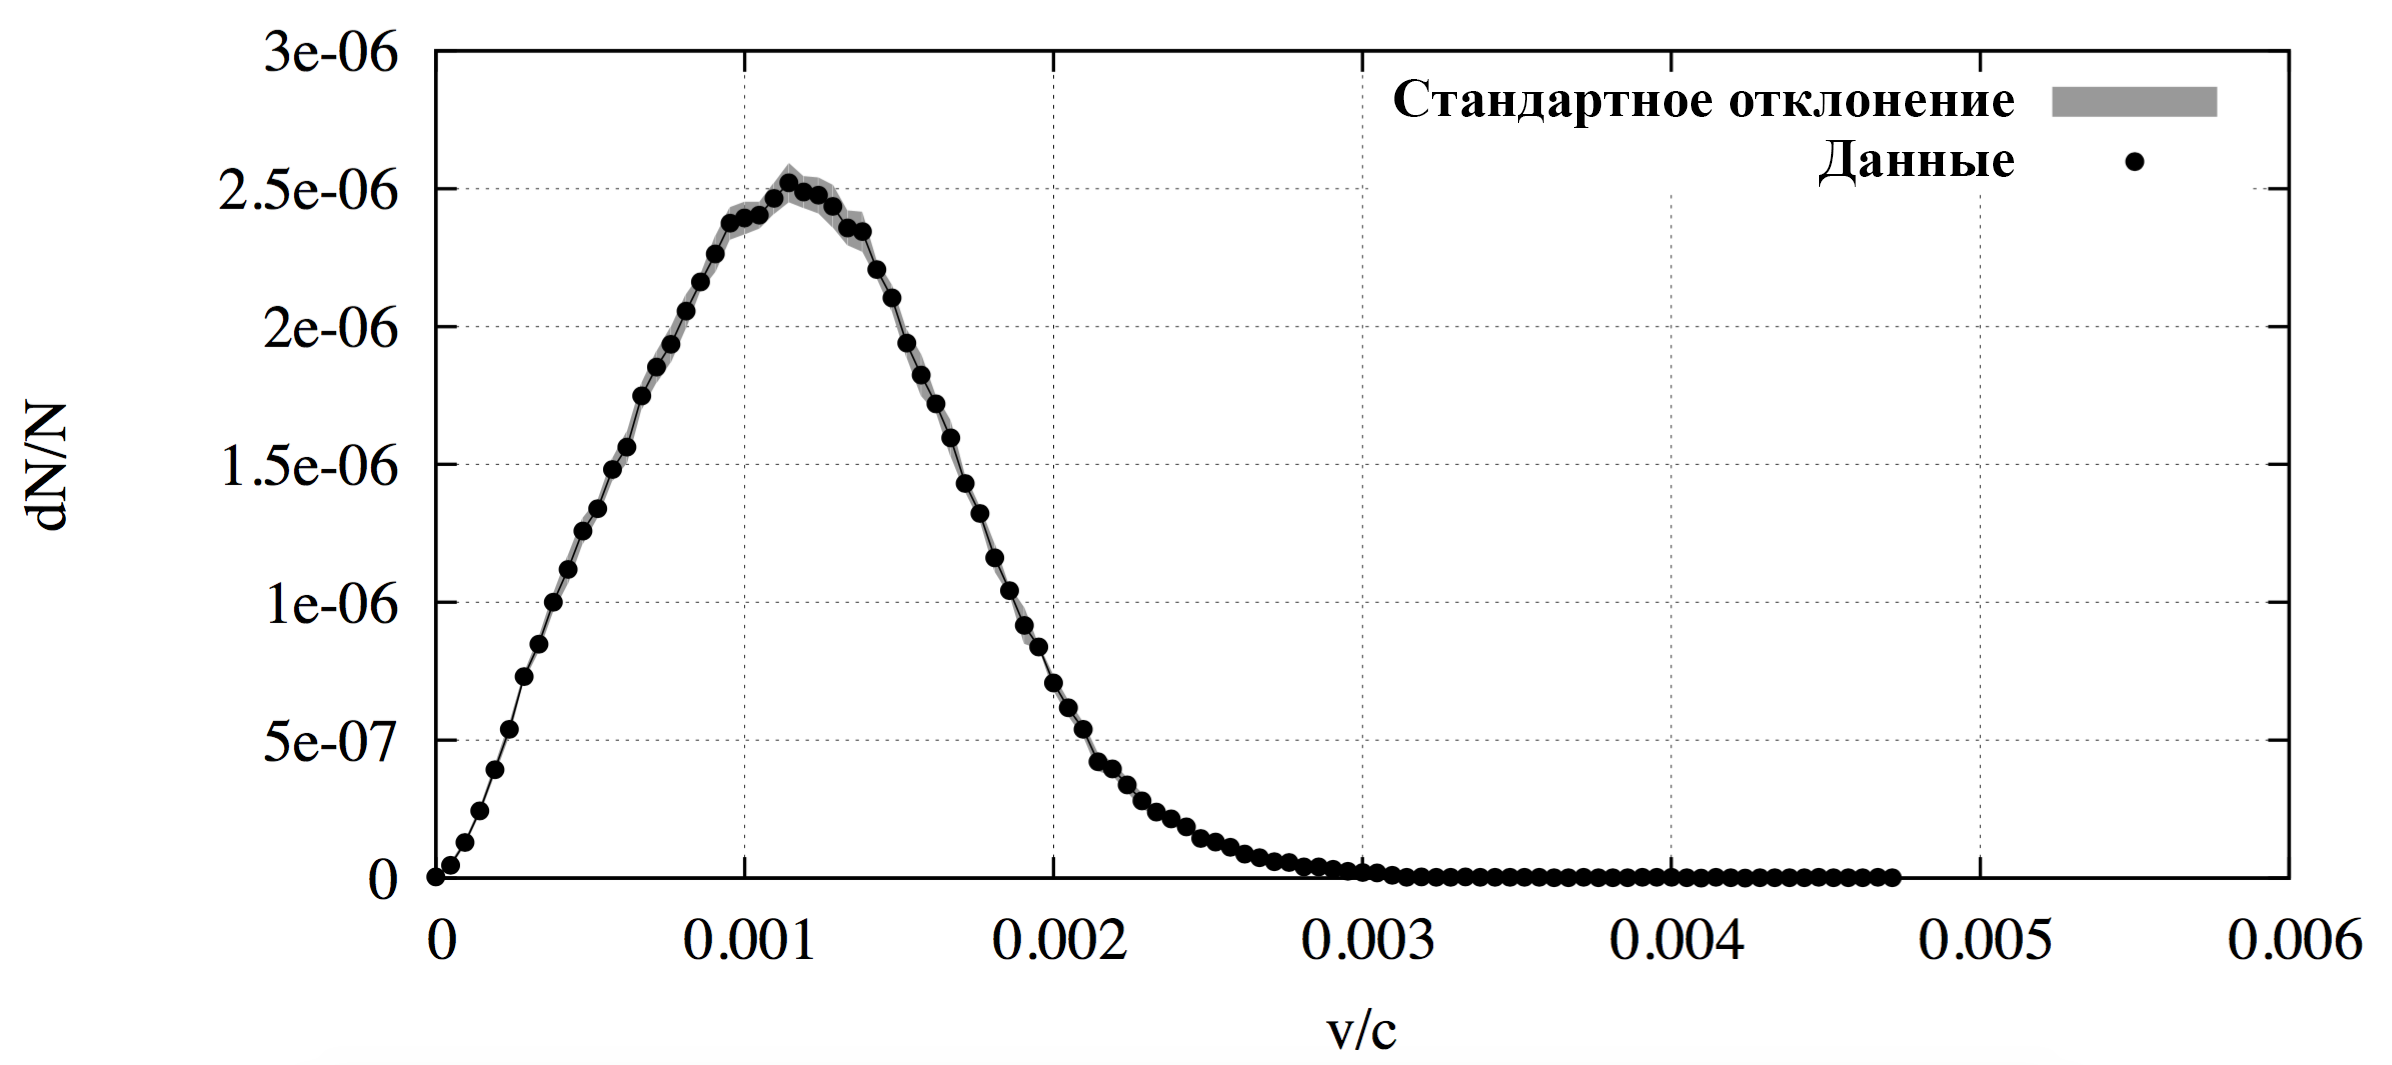
\includegraphics[width=0.75\linewidth]{fig/ch5/maxwell}
	\caption{Распределение ионов по скоростям}
	\label{fig:maxwell}
\end{figure}


\subsection{Сравнение экспериментов с инжекцией и без инжекции горячих ионов}

Ощутимая разница наблюдается только на графиках радиальной плотности (рисунок \ref{fig:density_r_w}). Без инжекции провал становится более плавный и без дополнительного локального минимума.

\begin{figure}[h!]
	\center
	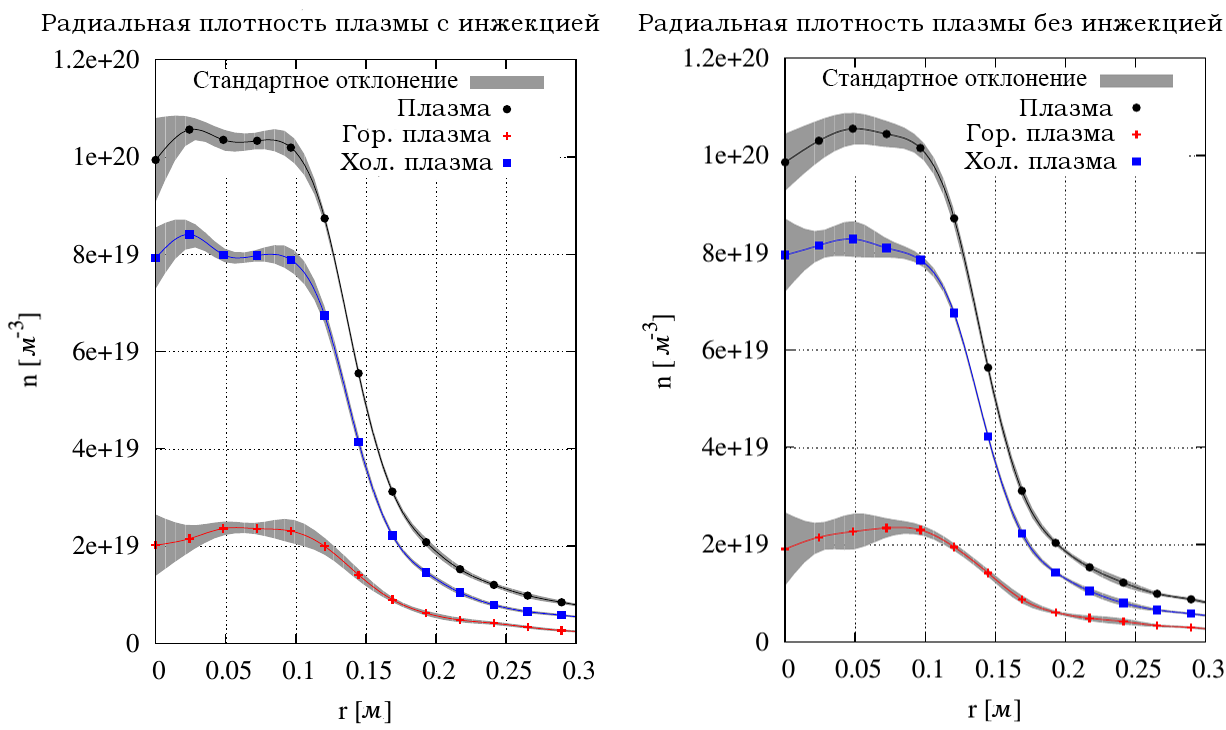
\includegraphics[width=1.\linewidth]{fig/ch5/density_comp}
	\caption{Радиальный профиль плотность плазмы при наличии и отсутствии инжекции}
	\label{fig:density_r_w}
\end{figure}

\section{Перспективы развития модели}

Построенная модель учитывает не все явления. Логическим продолжением развития данного исследования может стать добавление учёта процессов ионизации и реакций термоядерного синтеза. Создание гибридной модели, учитывающей как движение электронов, так и движение ионов, причём делать это пошагово --- при движении электронов считать ионы неподвижными, а при расчёте ионов добавлять экранирующую функцию. Каждый шаг возможно будет связать с предыдущим рассчитанными распределением потенциала. Кроме того, необходимо учесть влияние металлических стенок конструкции, а также множество дополнительно установленных систем стабилизации, например созданное радиальное электрическое поле для подавление МГД неустойчивости и уменьшения радиальных потерь.

Также с помощью полученных данных, возможно уже получить начальные распределения $n(\vec{r})$ для более сложных вычислений.